\section{Background}\label{background}

One of the most impactful uses of AI in healthcare is clinical decision
support.Clinical decision support is one of the most impactful uses of
AI in healthcare. Fluently capturing the meaning of medical questions
seems to be within reach of large language models (LLMs). They contain a
tremendous amount of book-learned and guidebook knowledge {[}1{]}
(reach). Yet fluency is not trustworthiness. There are two failure modes
which prevent the safe deployment. First, LLMs hallucinate---they
generate well-developed claims which are not grounded in any text
sources {[}2{]}. Second, a clinician was not easily able to determine
the level of confidence or the source for an answer but based on
evidence or what appeared to be evidence, rather than on which actual
documents were decisive. Retrieval-augmented generation (RAG) {[}3{]}
solves the first failure mode as such; conditioned as follows: Nowadays,
it is commonplace to find generation on retrieved documents. Modern
systems combine sparse lexical scoring (BM25 {[}4{]}) together with
dense bi-encoders {[}5{]} to fuse the rankings {[}6{]} and re-rank the
results with cross-encoders {[}7{]}. But the standard model -- retrieve
concatenate generate -- still exists reactive: it removes the notion of
a context window in the retrieved passages treating them as static and
delegates any reasoning to it. It was interesting to discover why the
self-assessment, and provenance are aspects to the opaque pass forward
by the LLM. For high-stakes clinical use, just using this will not do.

\section{Rationale of the Study or
Motivation}\label{rationale-of-the-study-or-motivation}

A good clinical AI system is based on three properties which are missing
from the canonical RAG pipeline. Prospective reasoning: good clinical
practice makes a simulative examination of what the patient is going to
do. He ought to consider the actions of the candidates before committing
to it. Calibrated self-knowledge system: a trustworthy system Answer a
question correctly with 0.95 confidence. Answer a question correctly
with 0.95 confidence/answer it incorrectly with 0.95 confidence not all
of the random variables at the edge of the training distribution are the
same. Checks for auditing purposes; Then, any system of accountability
should specify on the document, which one was pivotal, not just say
documents. decoratively. According to this thesis, these three
properties can be achieved by a rephrasing of the problem: around two
mechanisms. Context labelling is a process of adding a structured,
machine-readable label. A retrieved set of evidence for each answer, a
set of causal knowledge-graph relationships consulted, a hypothesized
state of diagnosis, along with a level of uncertainty calibrated.
Original-source tracking then shares a linkage of each claim to the
corresponding document(s), aggregating contributions of each document
according to Shapley value attribution. These, along with other
mechanisms, transform into or combine with making an opaque generator
auditable, calibrated and source-grounded to become a helping assistant.

\section{Problem Statement}\label{problem-statement}

An answer to a clinical query q and a corpus of medical documents should
be generated with the aim of producing an answer that is (a) based on
retrieved evidence, (b) with the appropriate level of confidence and an
explicit statement,(c) uncertainty due to the specific source documents
used to determine. A forward simulation of the patient's diagnostic
trajectory as opposed to (d) it, informed by a forward simulation of the
patient's diagnostic trajectory. One single front end of variables, and
a depth gain in the value of the problem.What we really need is a system
that gives us an answer as well as a set of variables, and some "depth
gain" in the value of the problem. Once a document is loaded, additional
labels, such as the ones mentioned below, are provided to help users
better read and interpret it: Attributing vector is compact enough to
easily train and audit on commodity hardware, yet powerful enough that
you can easily generate attributive explanations from the network.

\section{Objective}\label{objective}

This work aims to set the goals as follow: 1. design and implement an
augmented hybrid retrieval framework using a RAG approach with an
included action-conditioned latent. e.g., world model for future
thinking and "Tree of Thought" planning; 2. generate calibrated
predictive uncertainty in an explicit epistematic/aleatoric
decomposition using a deep ensemble; and 3. develop original-source
tracking with Shapley-value based evidence attribution and explicit
knowledge citations; 4. have a compact and trainable neural core (∼10M
parameters) that takes less than 20 minutes to train on one consumer
graphic processing unit; 5. analyze the trustworthiness using
calibration, generalisation, statistical significance and a strong RAG
baseline controlled comparison; and 6. describe its area of operation
and weaknesses responsibly, so as to ensure one can interpret it
correctly.

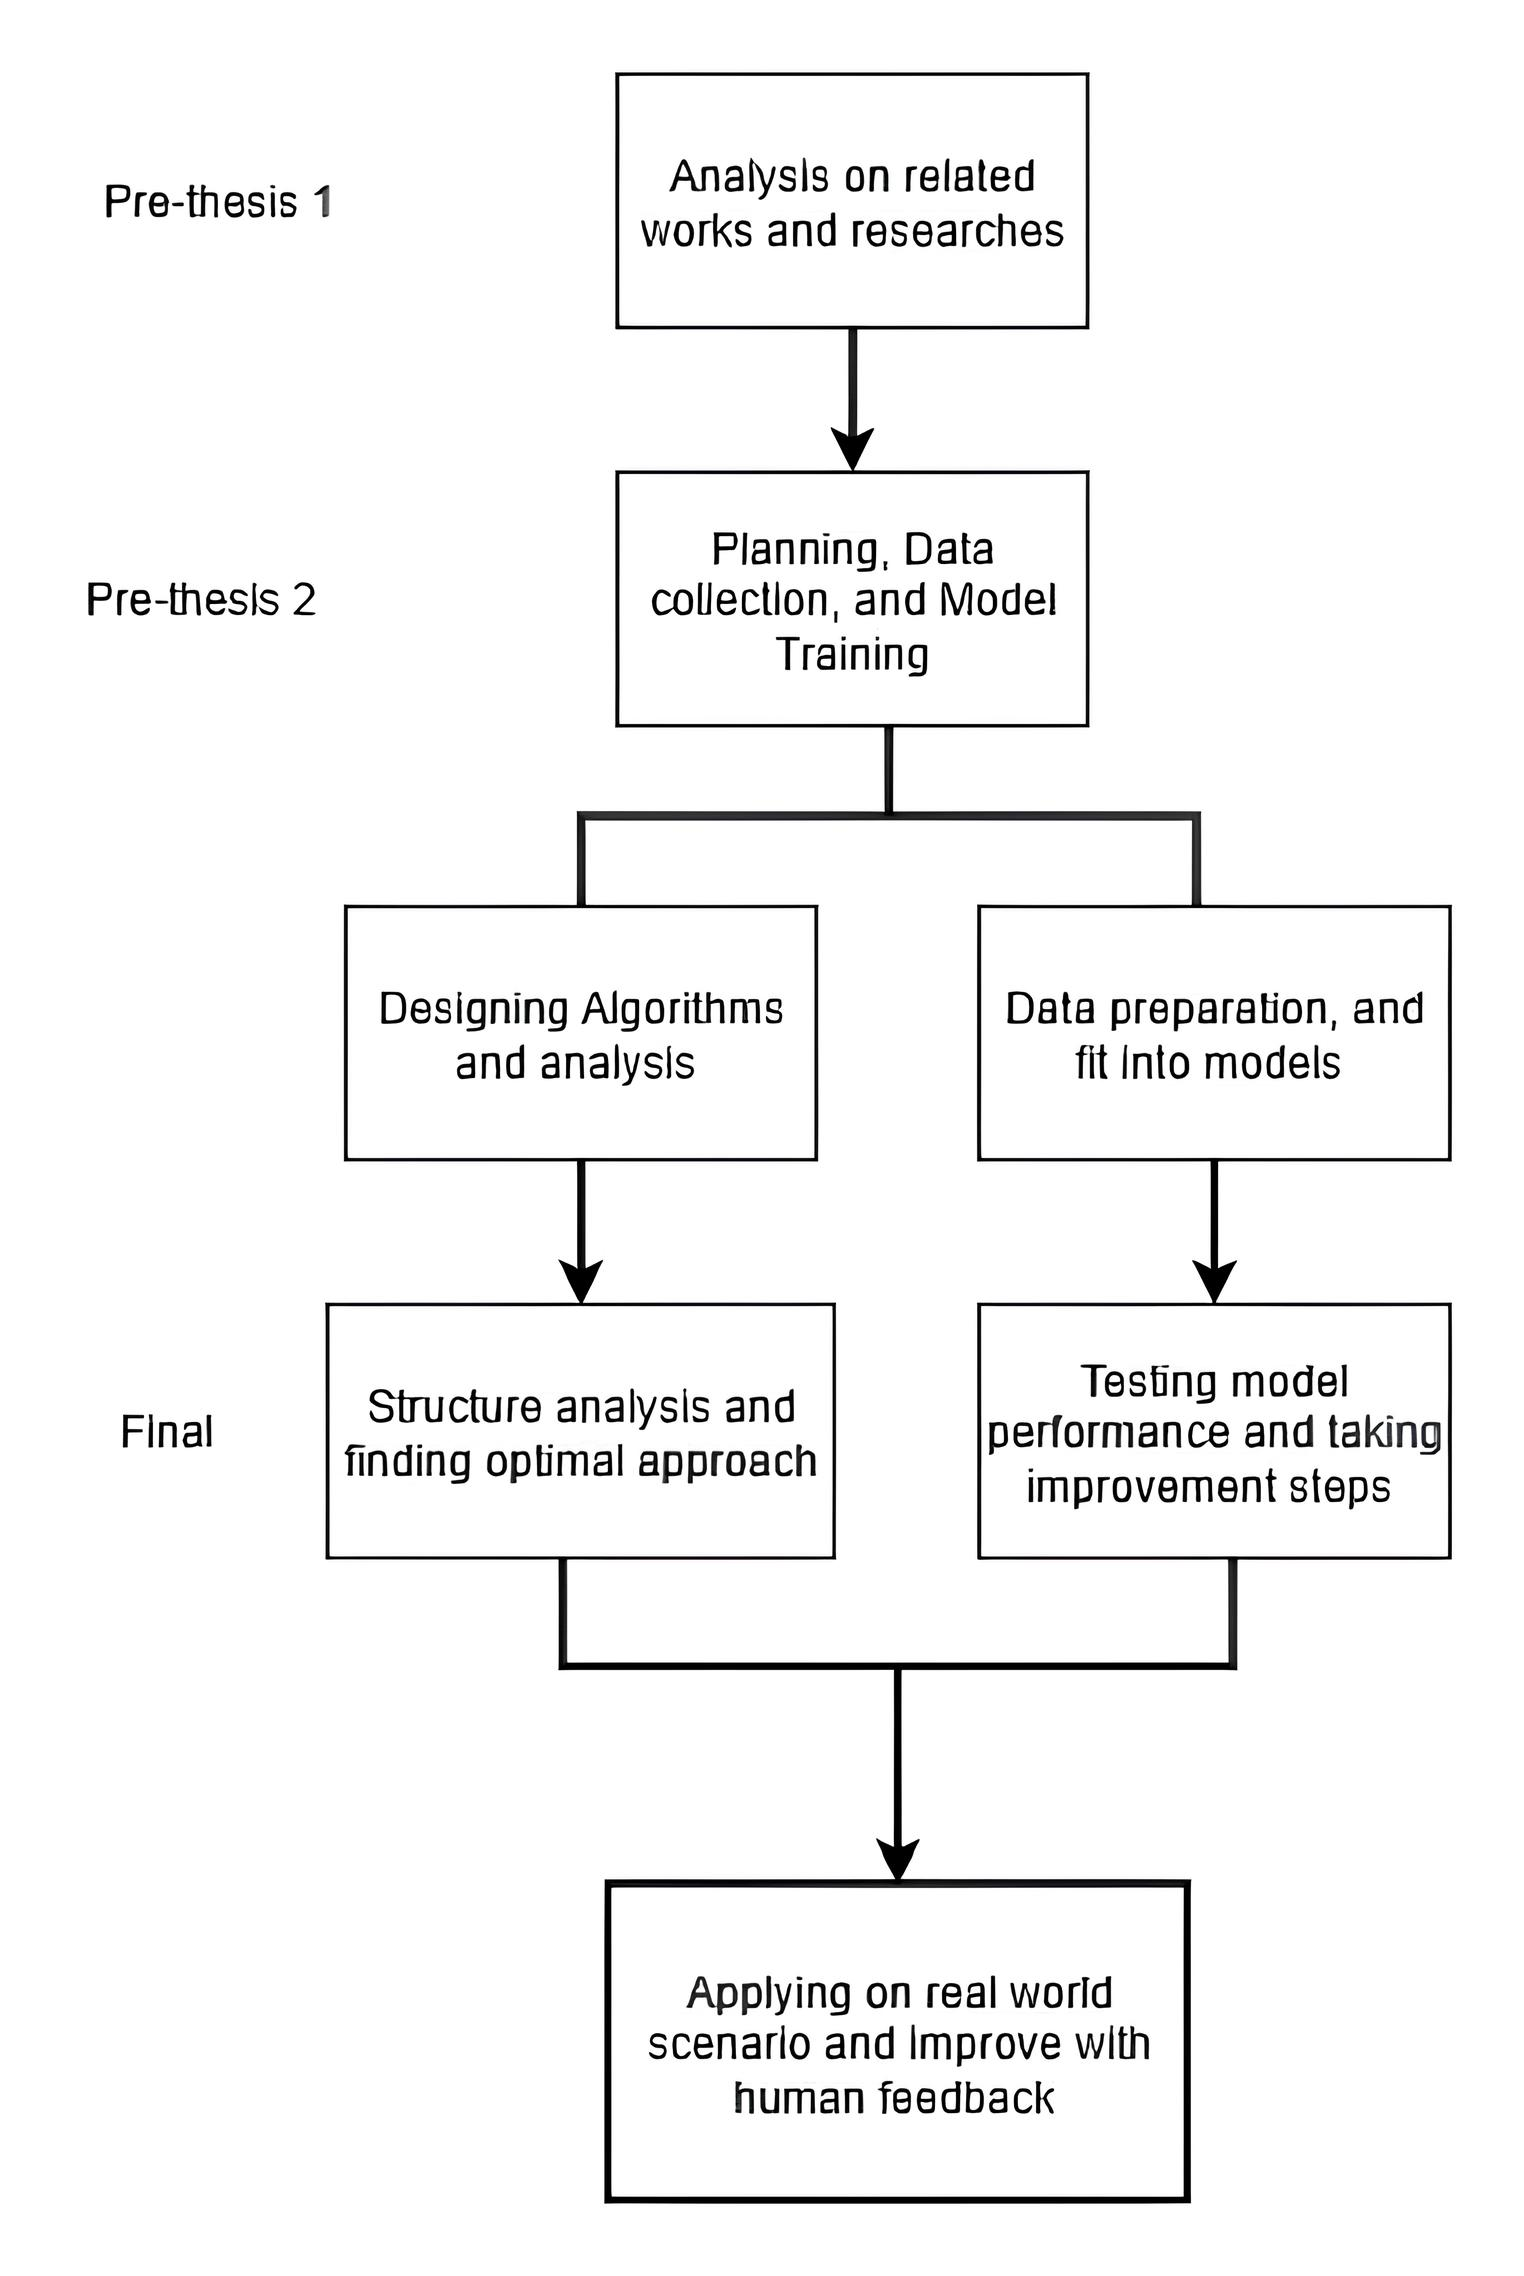
\includegraphics{images/timeline.jpg}

Project Timeline

\section{Methodology in Brief}\label{methodology-in-brief}

The proposed framework is based on a 12 stage pipeline broken down into
five functional blocks : retrieval, graph reasoning, world-model
planning, uncertainty and explanation (Fig. 1.1). A hybrid retrieval and
re-ranking is used to expand and answer a query, and grounded evidence
is produced. A latent patient state which has multiple other instances
of encoded knowledge, such as and a causal knowledge graph, is rolled by
its latent world model. The result is then sent to the state forward
under a beam planner based on a tree of thought; a deep ensemble is used
to score the result. The uncertainty is ordered; the draft is checked by
a "hallucination" check; and a module acting according to the "Shapley
values" is used to check the draft. Gives credit to individual documents
prior to LLM verbalizing the final, source tracked response. Various
shapes of the tensors are located in the detailed neural architecture,
as illustrated in Figure 1.2. Labels such as context labels come into
and constitute source tracking.

Figure1.1: Inference pipeline used for the generation of trustworthy
clinical question answering. The query is expanded with some extra
terms, This is answered by using hybrid retrieval and re-ranking and
encoded by the causal knowledge-graph GNN into a latent state, forwarded
by the latent world model with a beam planner tree-of-thoughts. Deep
ensemble score values of calibrated uncertainty were used and verified
for hallucination attributes. We finally get evidence through Shapley
values, and then, explicitly tracked by the LLM quantitatively.

Figure1.2: Detailed neural architecture, designed as tensor shapes are
shown in figure 1.2. Context labels (observations of patients),
relationships, and probability distributions (inference labels) come in
on the left; the causal GNN, evidence-fusion relationships, and
probability distributions (inference labels) enter on the left. All of
the 10.1M parameter core encoder, action-conditioned causal residual,
recurrent latent dynamics, in addition to the right-hand heads, beam
planner, deep ensemble and Shapley sourcetracking module, yield a
calibrated, sourced answer.

\section{Scope and Challenges}\label{scope-and-challenges}

The focus of this thesis is the design, implementation and evaluation of
the trust mechanisms The context labelling and source tracking
capabilities and world-model core that supports them, were evaluated All
resources on public clinical-QA resources. The work is influenced by a
number of hurdles. The effects of the system dynamics are addressed.
With semi-synthetic trajectories, which were created by deconstructing
the evidence step-by-step, the relationships between the variables
involved with the target are very close to being deterministic. The
actions do not refer to evidence acquisition but rather to actions that
should be taken physical interventions. The knowledge graph stores a
stochastic causal prior, rather than a curated ontology. MacroF1 is a
challenging metric as it is based on fine-grained and imbalanced rank
classes over 49 pathologies. We make every of these as an explicit
boundary of credit instead of a hidden boundary of credibility, and not
as an absolute boundary of finitability. We will come back in Sections
5.6 and 6.3, and you will assume this as a prerequisite.
